\documentclass[final]{beamer} % Layout
\usepackage[size=a1,orientation=portrait]{beamerposter} % Main layout class
\usepackage{graphicx} % Include graphics
\usepackage{textpos} % Position blocks of text into columns
\usepackage{hyperref} % Make URLs clickable
\usepackage{multicol} % Multiple columns
\usepackage[utf8]{inputenc} % Handle UTF8 input in this source
\usepackage{helvet} % Use helvitica as main font
\usepackage{palatino}
\usepackage{subcaption} % For subfigure environment for side by side figures
\usepackage[mathscr]{eucal} % For \mathscr

%----------------------------------------------------------------------------------------
%	PACKAGE OPTIONS
%----------------------------------------------------------------------------------------
\mode<presentation>
\usetheme{bristol}

\setlength{\TPHorizModule}{\paperwidth}
\setlength{\TPVertModule}{\paperheight}
\setlength{\parskip}{1em}

%----------------------------------------------------------------------------------------
%	TITLE SECTION
%----------------------------------------------------------------------------------------
\title{Feature analysis of two stream CNNs for action recognition}
\author{Will Price (\texttt{wp13824@bristol.ac.uk}), Dima Damen (\texttt{csxda@bristol.ac.uk})}
\institute{University of Bristol}
\date{\today}
%----------------------------------------------------------------------------------------
\newcommand{\etal}{\textit{et al.}}
\newcommand{\learningrate}{\eta}
\newcommand{\neuron}[2]{a_{#2}^{(#1)}}
% 1: layer index
% 2: neuron index
\newcommand{\neuronforward}[2]{\hat{a}_{#2}^{(#1)}}
% 1: layer index
% 2: neuron index
\newcommand{\ebpscalar}[2]{Z_{#2}^{(#1)}}
% 1: layer index
% 2: neuron index
\newcommand{\weight}[3]{w_{#2,#3}^{(#1)}}
% 1: layer index
% 2: from neuron index
% 3: to neuron index
\newcommand{\children}[2]{\mathscr{C}^{(#1)}_{#2}}
% 1: layer index
% 2: neuron index
\newcommand{\parents}[2]{\mathscr{P}^{(#1)}_{#2}}
% 1: layer index
% 2: neuron index
\newcommand{\cwp}[4]{P\left(\neuron{#1}{#2} | \neuron{#3}{#4}\right)}
% 1: child layer index
% 2: child neuron index
% 3: parent layer index
% 3: parent neuron index
\newcommand{\mwp}[2]{P\left(\neuron{#1}{#2}\right)}
% 1: layer index
% 2: neuron index
\newcommand{\neuroninput}[2]{\tilde{a}^{(#1)}_{#2}}
% 1: layer index
% 2: neuron index
\newcommand{\neuronoutput}[2]{\hat{a}^{(#1)}_{#2}}
% 1: layer index
% 2: neuron index

\begin{document}
\begin{frame}[t] % The whole poster is enclosed in one beamer frame
  \setbeamertemplate{caption}{\raggedright\insertcaption\par}
  \addtobeamertemplate{block end}{}{\vspace*{1ex}} % White space under blocks
  \addtobeamertemplate{block alerted end}{}{\vspace*{2ex}} % White space under highlighted (alert) blocks
  \setlength{\belowcaptionskip}{2ex} % White space under figures
  \setlength{\belowdisplayshortskip}{2ex} % White space under equations

    \begin{alertblock}{Abstract}
      Convolutional neural networks (CNNs) recently achieved state of the art
      performance in object detection but their lack of transparency makes them
      difficult to debug and understand. Towards solving this problem, a
      technique, \textbf{excitation backpropagation (EBP)}, has been developed to
      determine which regions in the input of an image excite arbitrary neurons
      in the network, this technique can help understand what a network has
      learnt and whether it has generalised or overfit specific examples.

      EBP has been used to inspect object detection networks, but not two stream
      CNNs, a CNN architecture for action recognition from video sequences.

      Can EBP produce interpretable results on two stream CNNs for action recognition?
    \end{alertblock}

    \begin{block}{Two stream CNN}
      Two stream CNNs for action recognition are formed of two separate networks
      whose results are `fused' together. One network operates on a single video
      frame considering \textit{spatial} information. the second receives
      \textit{temporal} information from a stack of optical flow frames.

      \vskip0.5cm
      \centering
      \includegraphics[width=\textwidth]{media/images/two-stream-cnn}
    \end{block}

    \begin{block}{Excitation Back-propagation}
      Excitation back-propagation (EBP) is a technique to determine the regions
      in the input of a network that contribute to the excitation of an
      arbitrary neuron. By understanding the regions exciting a neuron we can
      infer certain features the network has learnt.
      \begin{figure}
        \begin{subfigure}{0.13\linewidth}
          \centering
          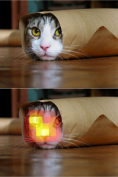
\includegraphics[height=13cm]{media/images/ebp-cat}

          EBP of `cat' neuron in an object detection CNN
        \end{subfigure}
        \begin{subfigure}{0.86\linewidth}
          \raggedleft
          \includegraphics[height=11cm]{media/images/ebp-example}

          \vspace{2cm}
          \centering
          EBP example on a network of fully connected layers
        \end{subfigure}
      \end{figure}
    \end{block}

    \begin{block}{Application of Excitation Back-propagation to two stream CNNs}
      \centering
      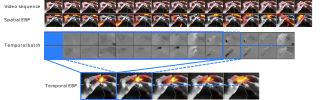
\includegraphics[height=16cm]{media/images/ebp-two-stream}
    \end{block}

    \begin{block}{Results}
      \centering
      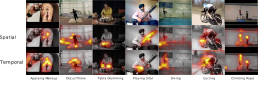
\includegraphics[keepaspectratio,height=20cm]{media/images/ucf101-ebp-results}
    \end{block}

  \begin{textblock}{0.49}(0.5, 0.64)
    \begin{alertblock}{Summary}
      \begin{itemize}
      \item Survey of methods for understanding CNNs.
      \item Excitation backpropagation applied to two stream CNN networks on the
        BEOID and UCF101 datasets.
      \item Contrastive attention works poorly on two stream CNNs compared to
        its superior results on CNNs for object detection.
      \end{itemize}
    \end{alertblock}

    \begin{block}{References}
    \end{block}
  \end{textblock}
\end{frame}
\end{document}
